\chapter{SNMP (Simple Network Management
Protocol)}\label{snmp-simple-network-management-protocol}

\section{SNMP Overview}\label{snmp-overview}

\begin{itemize}
\tightlist
\item
  SNMP is an INDUSTRY-STANDARD FRAMEWORK and PROTOCOL that was
  originally released in 1988
\end{itemize}

These RFCs make up SNMPv1 (Do not need to memorize)

\begin{lstlisting}
RFC 1065 - Structure and identification of management information for TCP/IP based internets
RFC 1066 - Management information base for network management of TCP/IP based internets
RFC 1067 - A simple network management protocol
\end{lstlisting}

\begin{itemize}
\tightlist
\item
  Don't let the `Simple' in the name fool you !
\item
  SNMP can be used to monitor the STATUS of DEVICES, make CONFIGURATION
  CHANGES, etc.
\item
  There are TWO MAIN TYPES of DEVICES in SNMP:

  \begin{itemize}
  \tightlist
  \item
    MANAGED DEVICES

    \begin{itemize}
    \tightlist
    \item
      These are the DEVICES being managed using SNMP

      \begin{itemize}
      \tightlist
      \item
        Ex: ROUTERS, SWITCHES
      \end{itemize}
    \end{itemize}
  \item
    NETWORK MANAGEMENT STATION (NMS)

    \begin{itemize}
    \tightlist
    \item
      The DEVICE / DEVICES managing the MANAGED DEVICES
    \item
      THIS is the SNMP `SERVER'
    \end{itemize}
  \end{itemize}
\end{itemize}

\section{SMNP Operations}\label{smnp-operations}

\begin{figure}
\centering
\pandocbounded{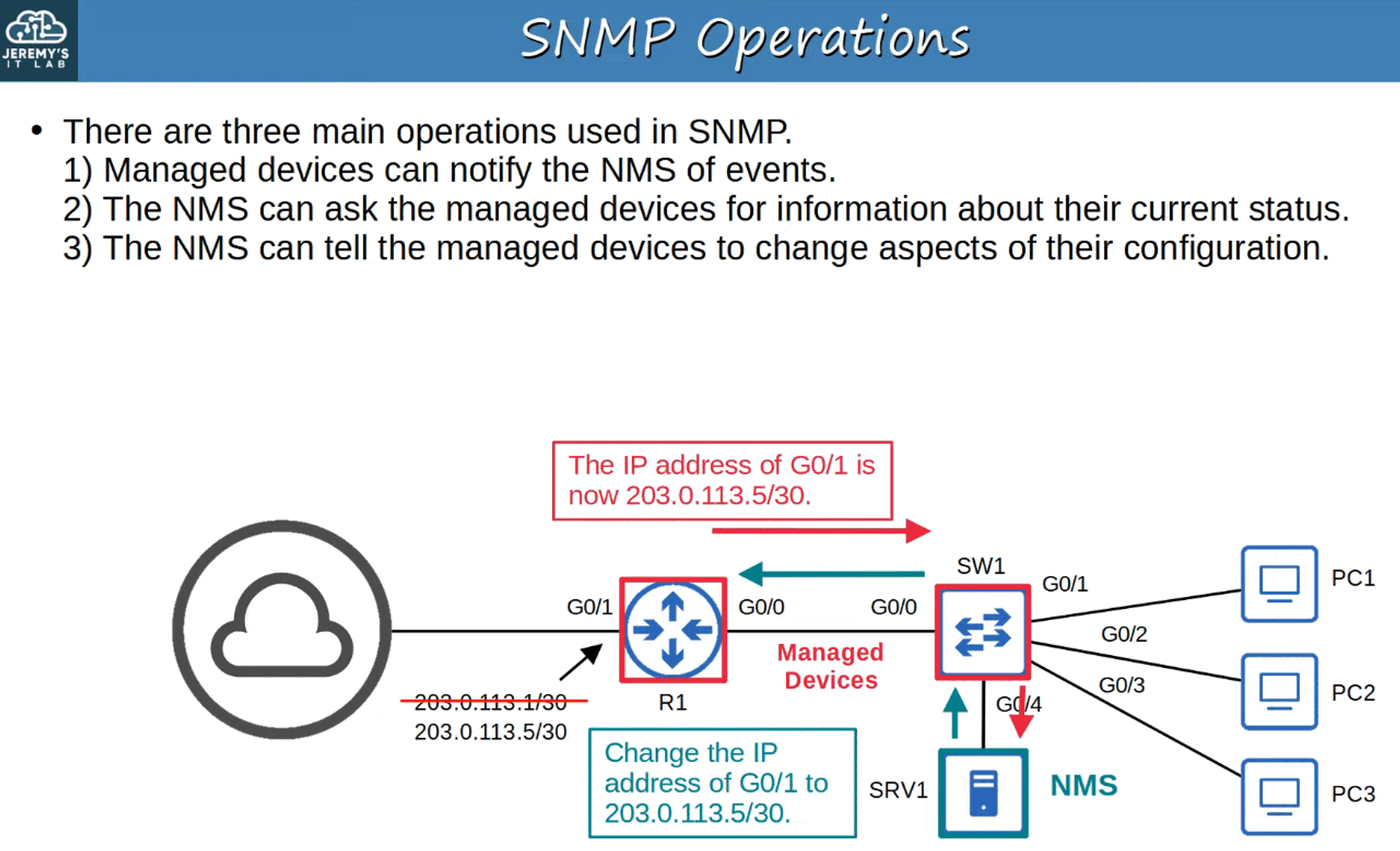
\includegraphics[keepaspectratio,alt={image}]{images/41-snmp/img-001.png}}
\end{figure}

\section{SMNP Components}\label{smnp-components}

\section{Overview}\label{overview}

\begin{figure}
\centering
\pandocbounded{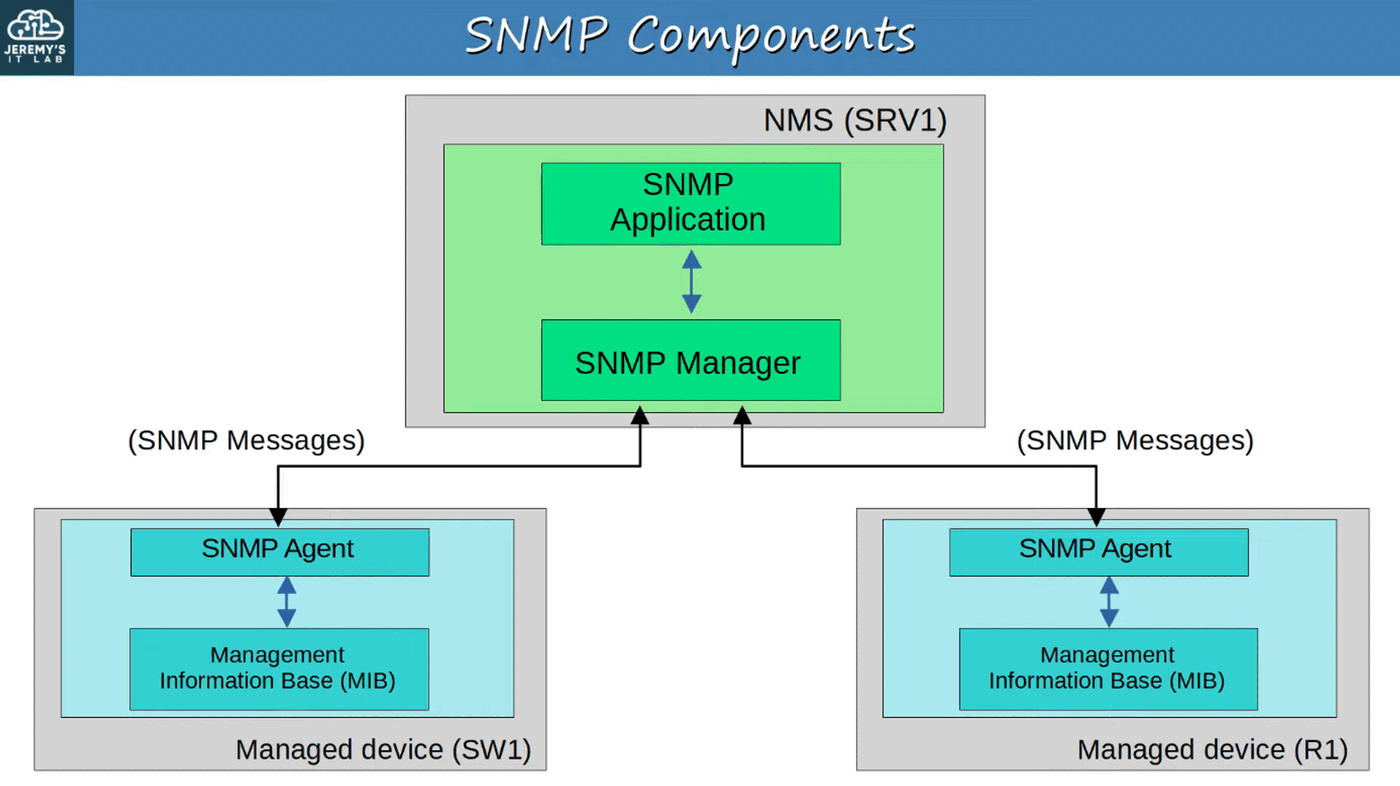
\includegraphics[keepaspectratio,alt={image}]{images/41-snmp/img-002.png}}
\end{figure}

\section{Nms}\label{nms}

\begin{figure}
\centering
\pandocbounded{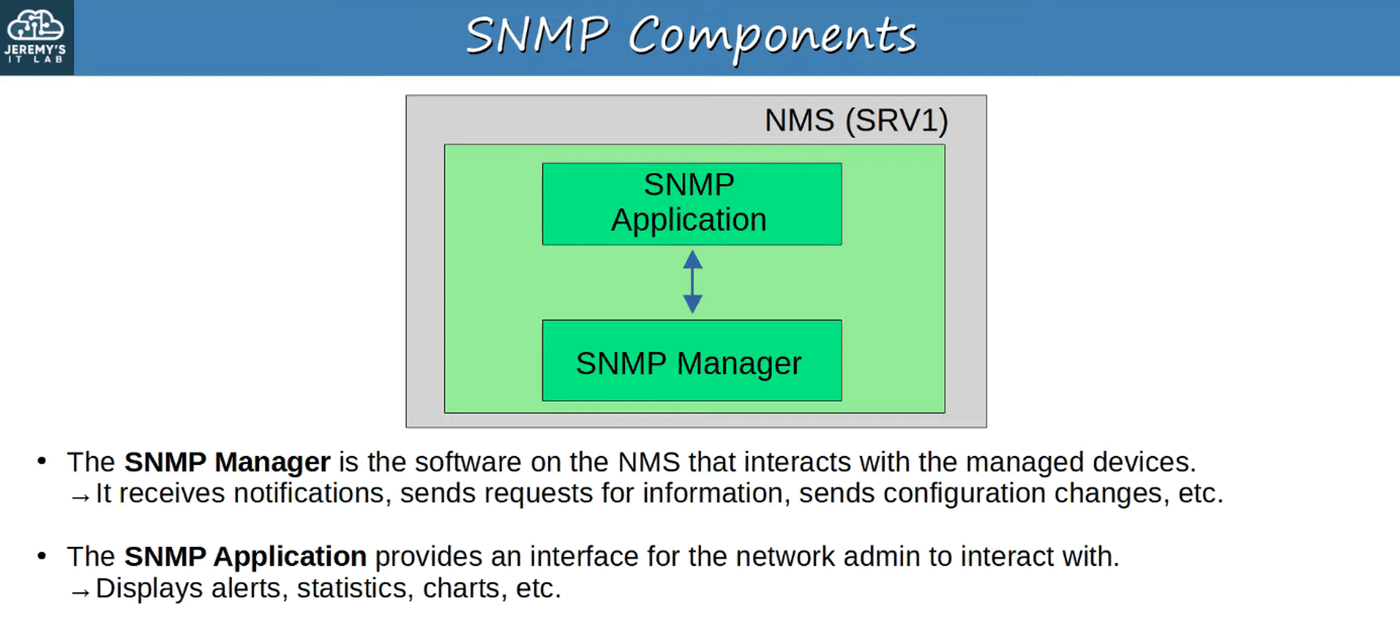
\includegraphics[keepaspectratio,alt={image}]{images/41-snmp/img-003.png}}
\end{figure}

\section{Managed Devices}\label{managed-devices}

\begin{figure}
\centering
\pandocbounded{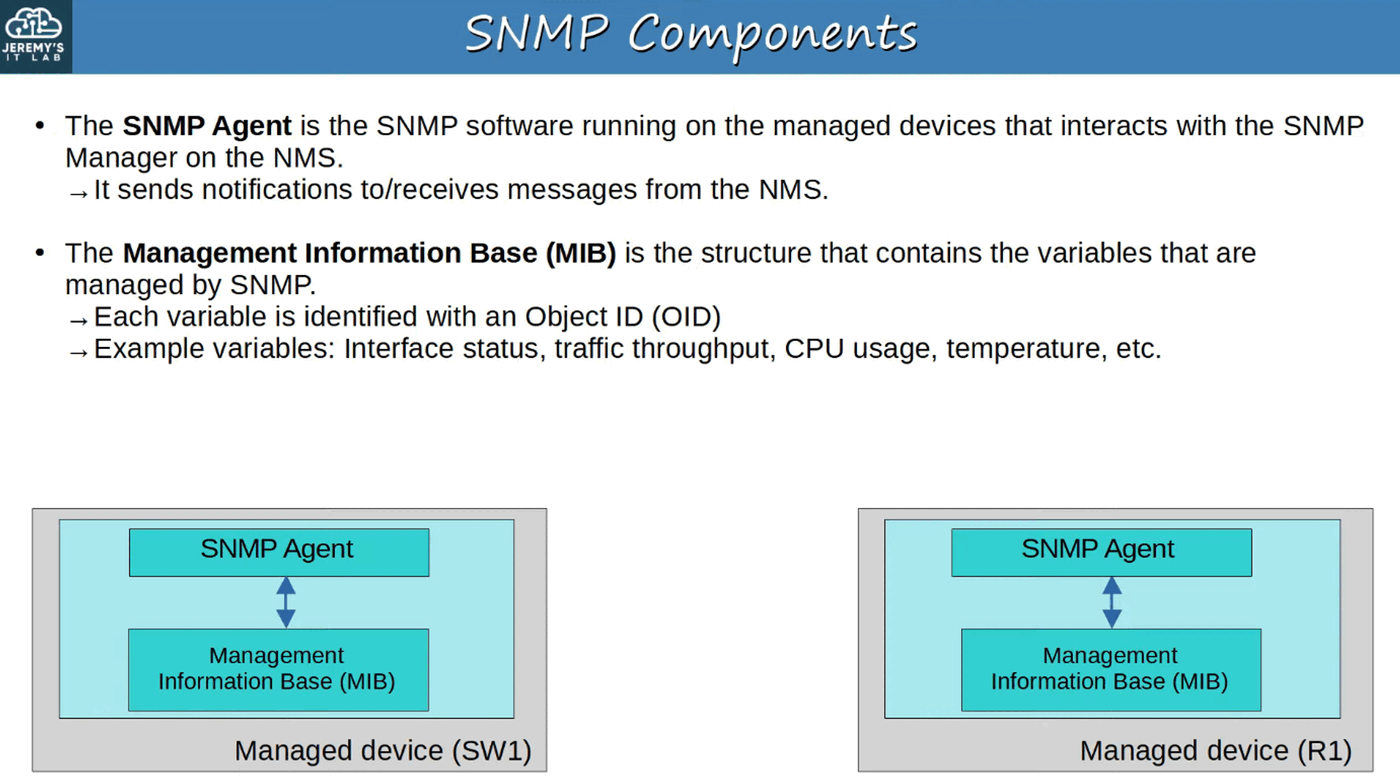
\includegraphics[keepaspectratio,alt={image}]{images/41-snmp/img-004.png}}
\end{figure}

SNMP OIDs

\begin{itemize}
\tightlist
\item
  SNMP Object IDs are ORGANIZED in a HIERARCHICAL STRUCTURE
\end{itemize}

\begin{figure}
\centering
\pandocbounded{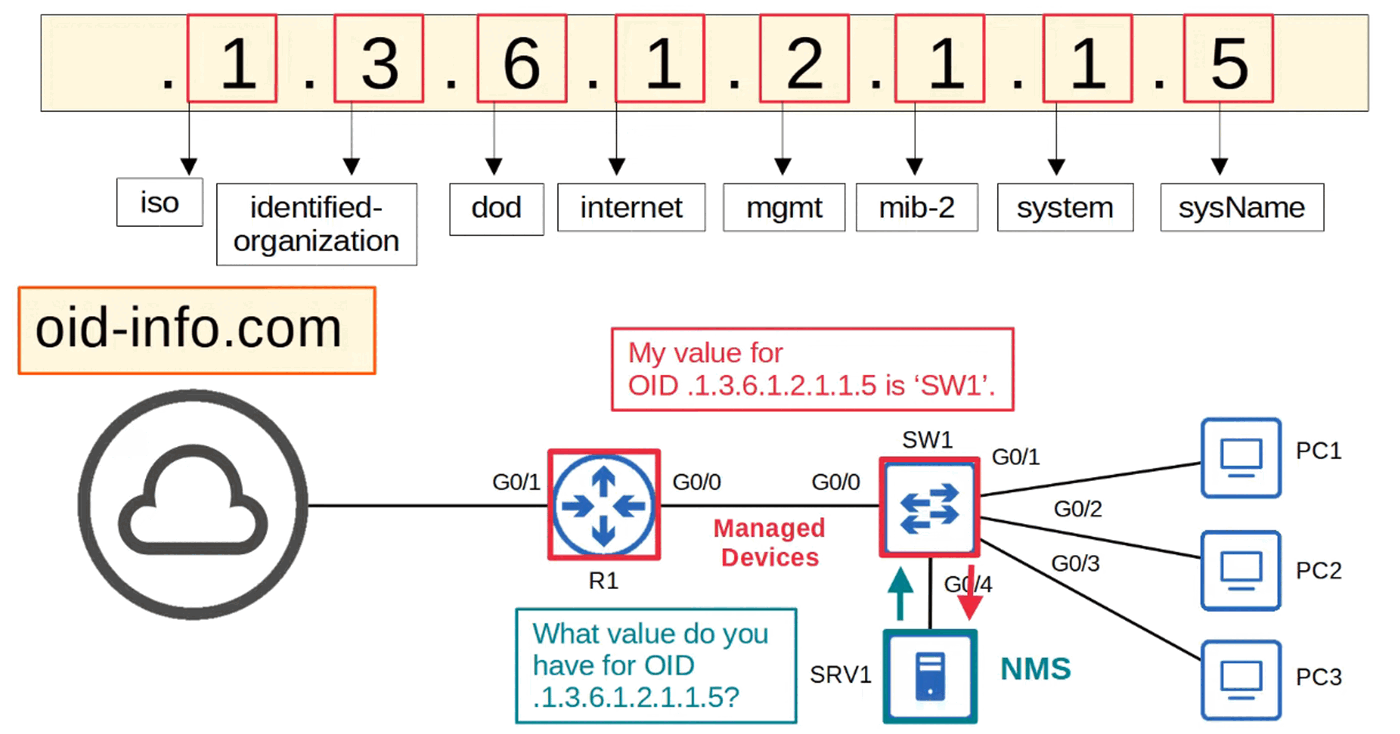
\includegraphics[keepaspectratio,alt={image}]{images/41-snmp/img-005.png}}
\end{figure}

\section{SNMP Versions}\label{snmp-versions}

\begin{itemize}
\item
  Many versions of SNMP have been proposed/developed, however, only
  three major versions have achieved wide-spread use:
\item
  \textbf{SNMPv1}

  \begin{itemize}
  \tightlist
  \item
    The ORIGINAL version of SNMP
  \end{itemize}
\item
  \textbf{SNMPv2c}

  \begin{itemize}
  \tightlist
  \item
    Allows the NMS to retrieve LARGE AMOUNTS of information in a SINGLE
    REQUEST, so it is more efficient
  \item
    `c' refers to the `community strings' used as PASSWORDS in SNMPv1,
    removed from SNMPv2, and then added BACK for SNMPv2
  \end{itemize}
\item
  \textbf{SNMPv3}

  \begin{itemize}
  \tightlist
  \item
    A much more SECURE version of SNMP that supports STRONG ENCRYPTION
    and AUTHENTICATION.
  \end{itemize}
\end{itemize}

\begin{tipbox}

WHENEVER POSSIBLE, this version should be used!

\end{tipbox}

\section{SNMP Messages}\label{snmp-messages}

\begin{figure}
\centering
\pandocbounded{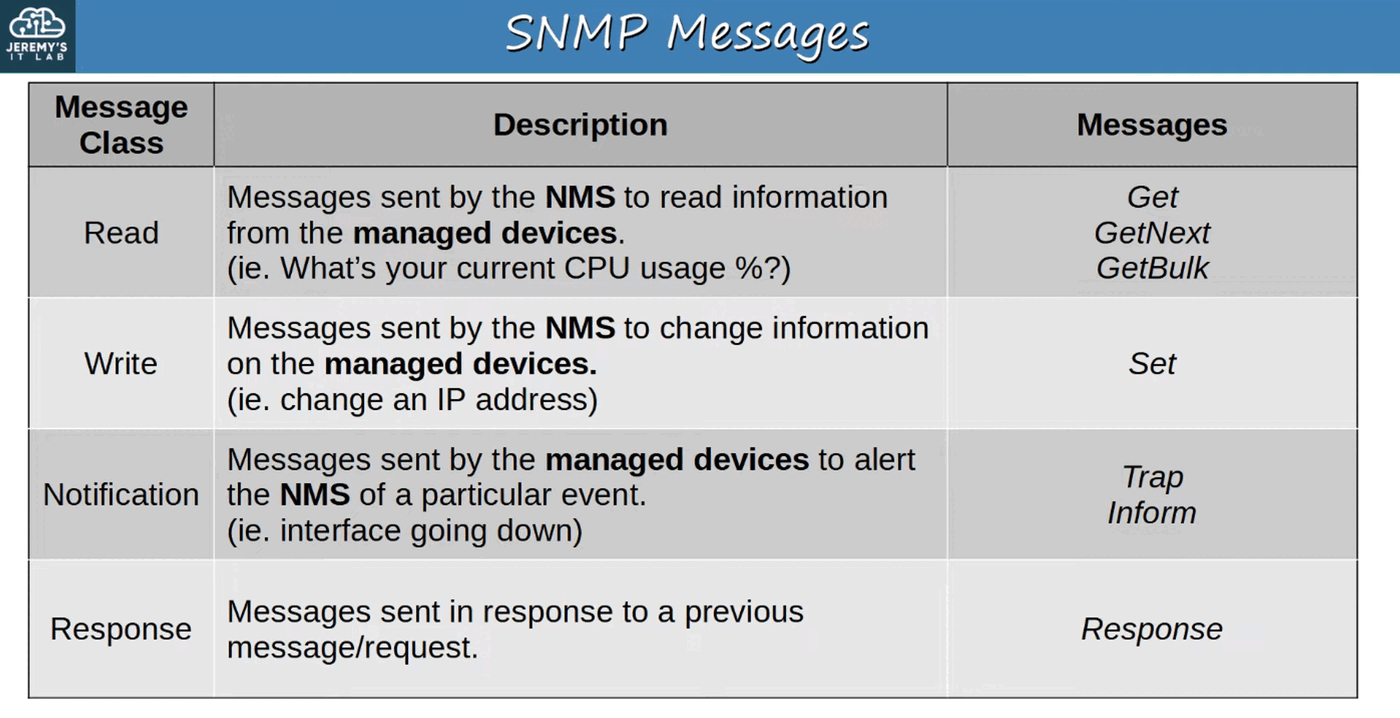
\includegraphics[keepaspectratio,alt={image}]{images/41-snmp/img-006.png}}
\end{figure}

\begin{enumerate}
\def\labelenumi{\arabic{enumi})}
\tightlist
\item
  SNMP READ
\end{enumerate}

\begin{figure}
\centering
\pandocbounded{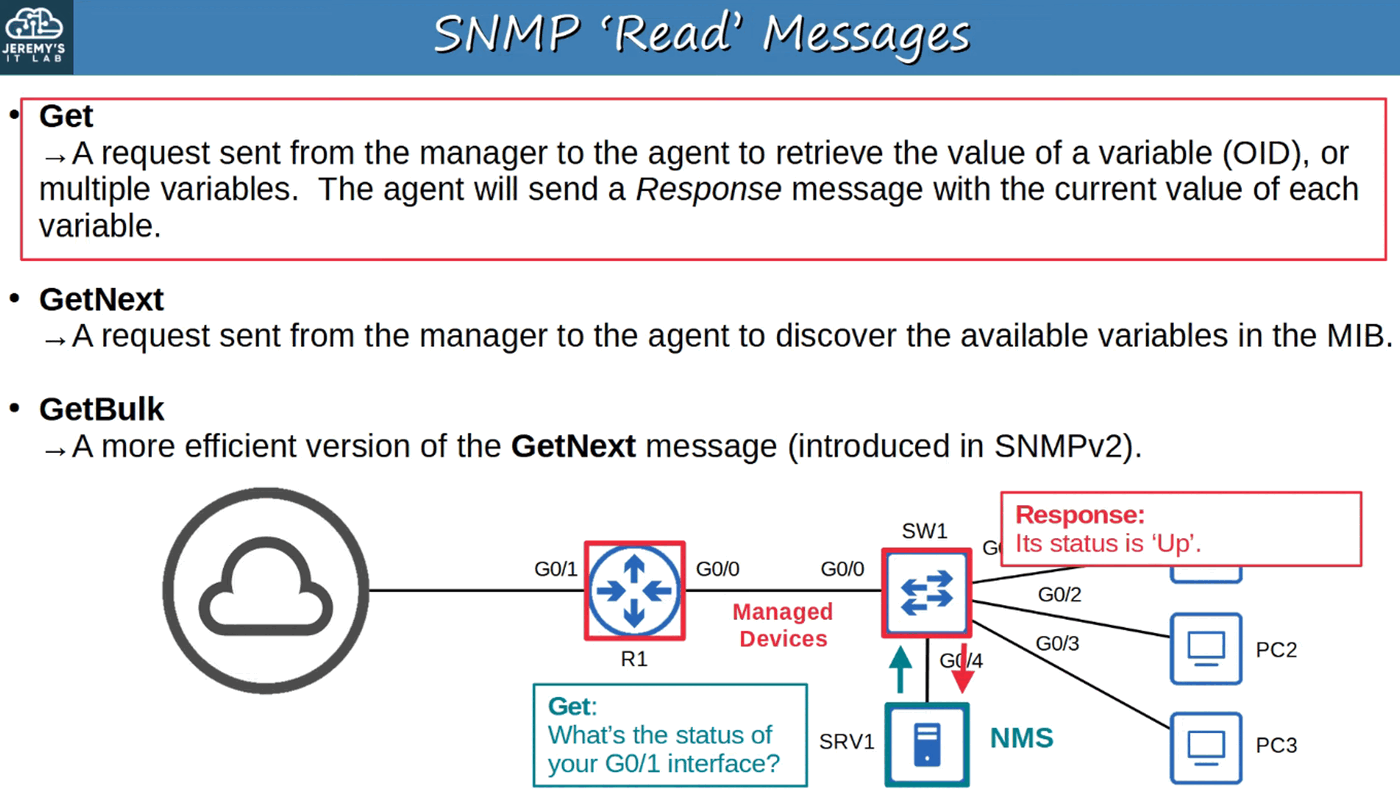
\includegraphics[keepaspectratio,alt={image}]{images/41-snmp/img-007.png}}
\end{figure}

\begin{enumerate}
\def\labelenumi{\arabic{enumi})}
\setcounter{enumi}{1}
\tightlist
\item
  SMNP WRITE
\end{enumerate}

\begin{figure}
\centering
\pandocbounded{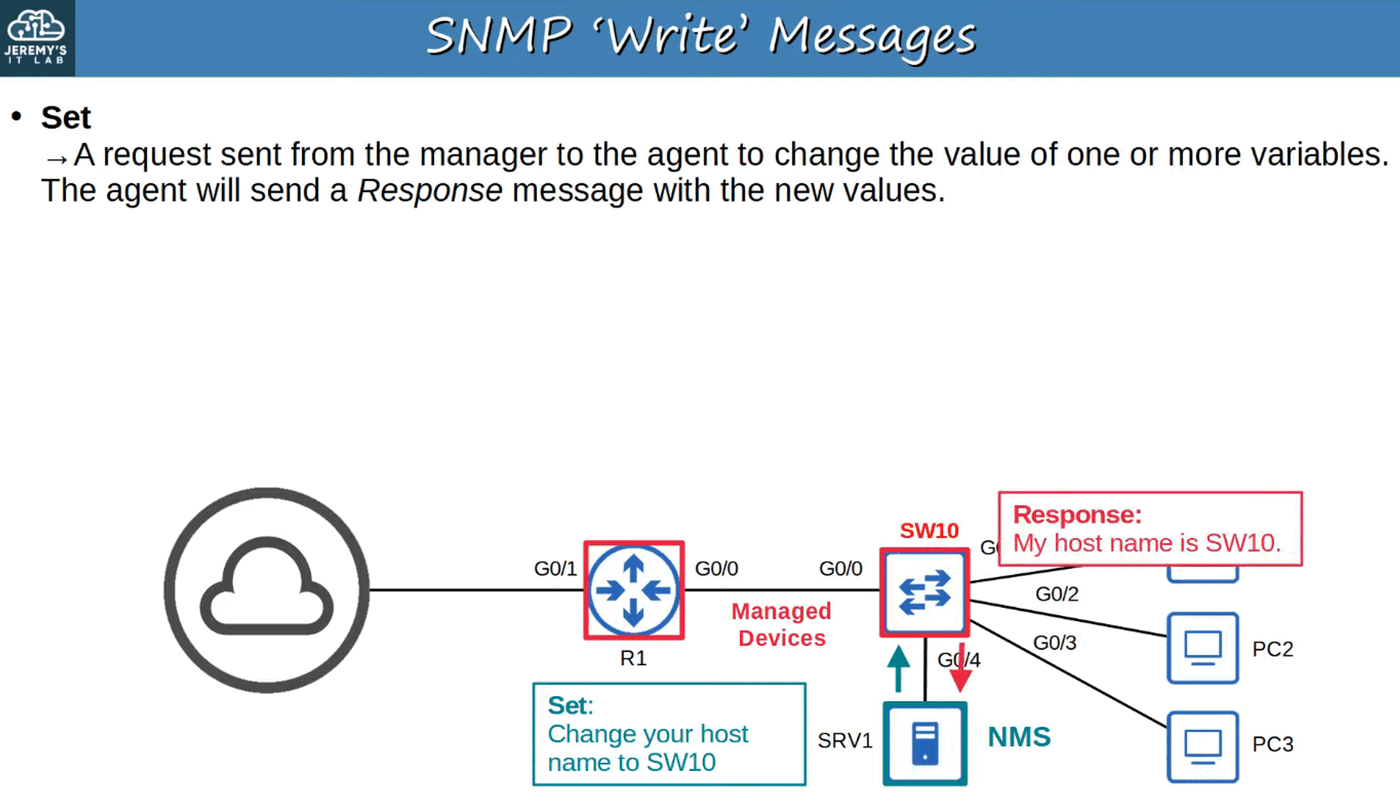
\includegraphics[keepaspectratio,alt={image}]{images/41-snmp/img-008.png}}
\end{figure}

\begin{enumerate}
\def\labelenumi{\arabic{enumi})}
\setcounter{enumi}{2}
\tightlist
\item
  SNMP NOTIFICATION
\end{enumerate}

\begin{figure}
\centering
\pandocbounded{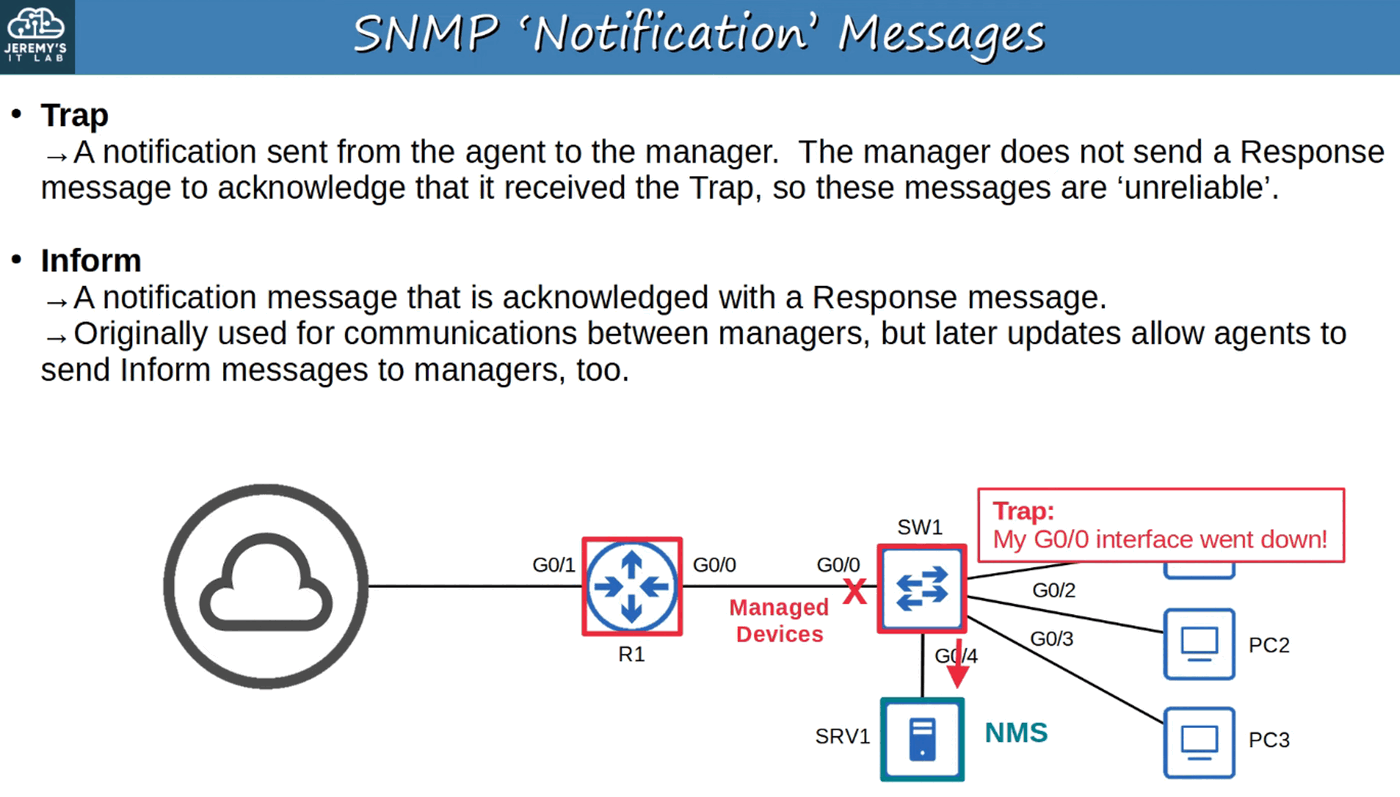
\includegraphics[keepaspectratio,alt={image}]{images/41-snmp/img-009.png}}
\end{figure}

SNMP AGENT listens for MESSAGES on UDP Port 161

SNMP MANAGER listens for MESSAGES on UDP Port 162

\begin{figure}
\centering
\pandocbounded{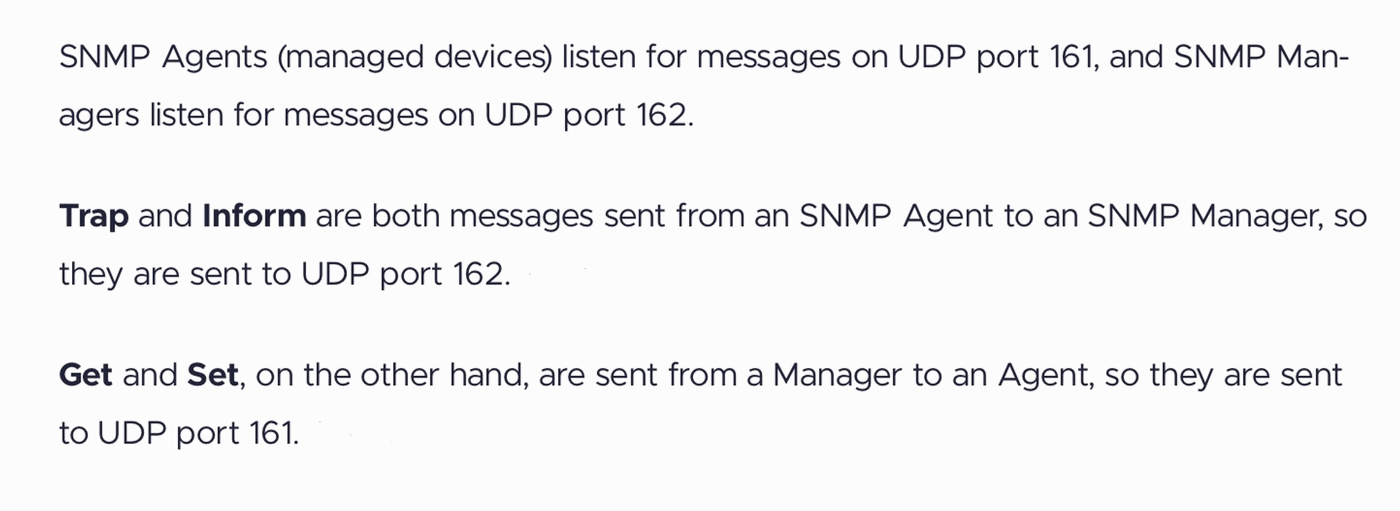
\includegraphics[keepaspectratio,alt={image}]{images/41-snmp/img-010.png}}
\end{figure}

SNMPv2c CONFIGURATION (Basic)

\begin{figure}
\centering
\pandocbounded{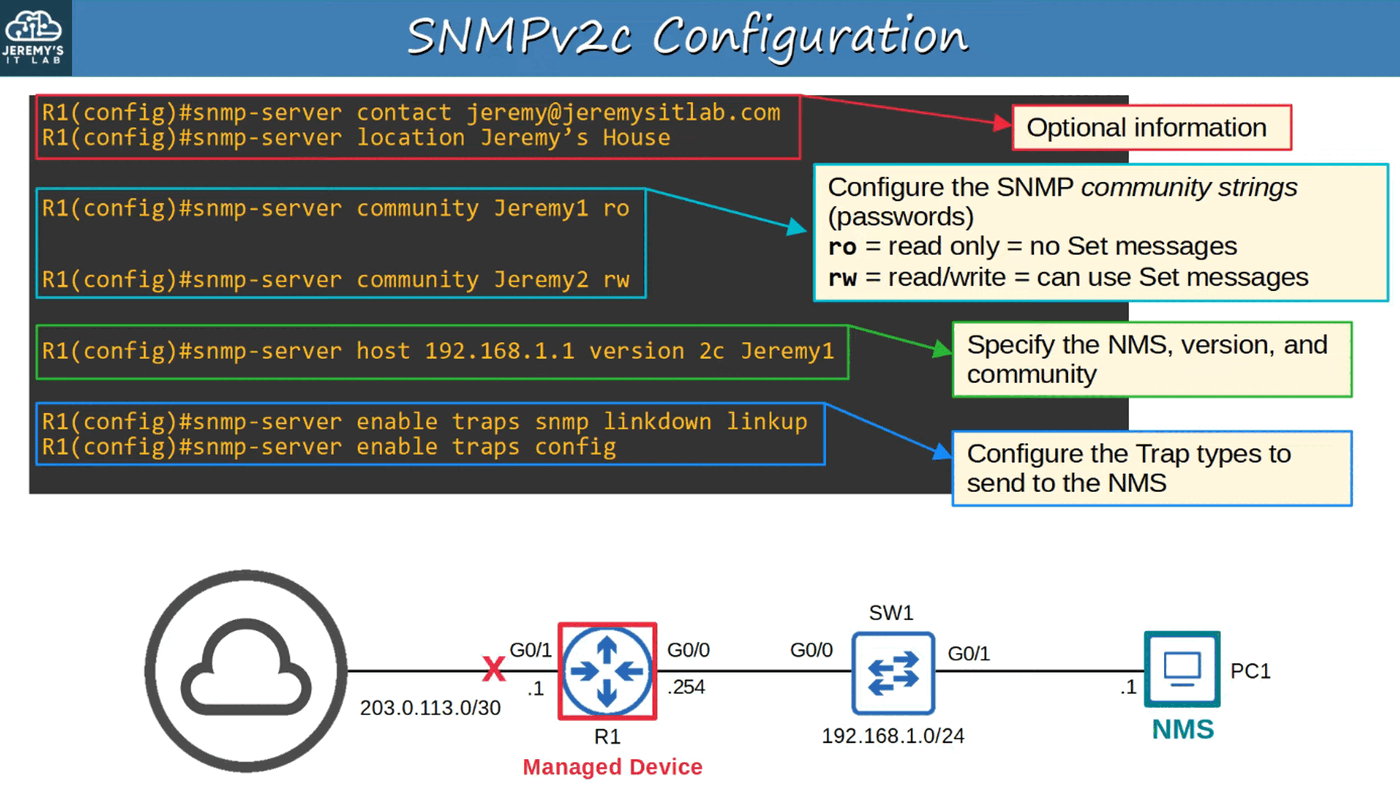
\includegraphics[keepaspectratio,alt={image}]{images/41-snmp/img-011.png}}
\end{figure}

WHAT HAPPENS WITH R1's G0/1 INTERFACE GOES DOWN?

\begin{figure}
\centering
\pandocbounded{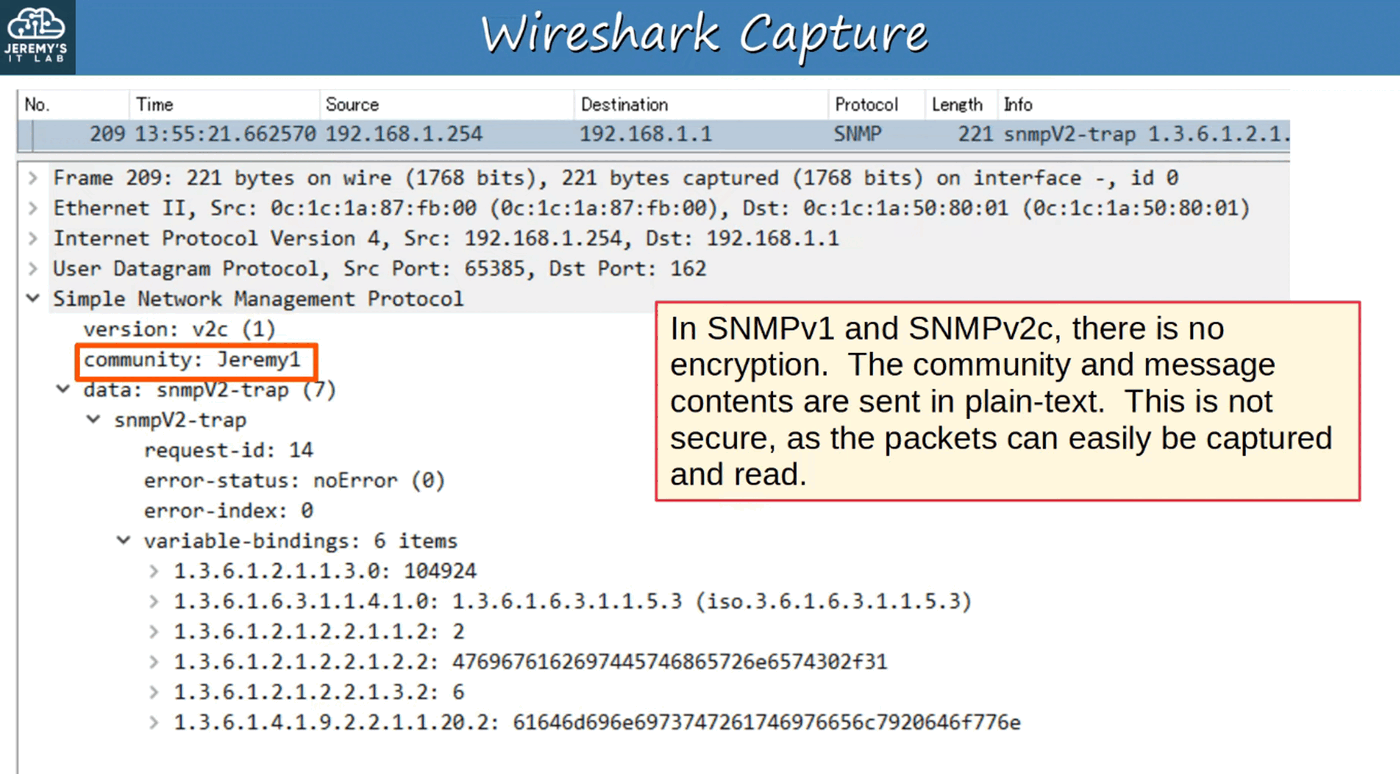
\includegraphics[keepaspectratio,alt={image}]{images/41-snmp/img-012.png}}
\end{figure}

\section{Note}\label{note}

UDP message sent to Destination Port 162 (SNMP Manager)

``version'' is set to v2c

community is ``Jeremy1'' (Read Only - no Set messages)

snmpV2-trap : trap message sent due to interface G0/1 going down

variable-bindings : contains the OID sent to identify the issue.

\section{SNMP Summary}\label{snmp-summary}

\begin{itemize}
\tightlist
\item
  SNMP helps MANAGE DEVICES over a NETWORK
\item
  MANAGED DEVICES are the devices being managed using SNMP (such as
  ROUTERS, SWITCHES, FIREWALLS)
\item
  NETWORK MANAGEMENT STATIONS (NMS) are the SNMP ``servers'' that manage
  the devices

  \begin{itemize}
  \tightlist
  \item
    NMS receives notifications from Managed Devices
  \item
    NMS changes settings on Managed Devices
  \item
    NMS checks status of Managed Devices
  \end{itemize}
\item
  Variables, such as Interface Status, Temperature, Traffic Load,
  Hostname, etc are STORED in the MANAGMENT INFORMATION BASE (MIB) and
  identified using Object IDs (OIDs)
\end{itemize}

Main SNMP versions : SNMPv1, SNMPv2c, SNMPv3

\begin{lstlisting}
SNMP MESSAGES :
* Get / GetNext / GetBulk
* Set
* Trap
* Inform
* Response
\end{lstlisting}
